\documentclass[a4paper,12pt]{article}
\usepackage[utf8]{inputenc}
\usepackage[spanish]{babel}
\usepackage{color}
\usepackage{parskip}
\usepackage{graphicx}
\usepackage{multirow}
\usepackage{listings}
\usepackage{vmargin}
\usepackage{datetime}
\newdate{date}{9}{11}{2017}
\graphicspath{ {imagenes/} }
\definecolor{mygreen}{rgb}{0,0.6,0}
\definecolor{lbcolor}{rgb}{0.9,0.9,0.9}
\usepackage{epstopdf}
\usepackage{float}


\setpapersize{A4}
\setmargins{2.5cm}       % margen izquierdo
{1.5cm}                        % margen superior
{16.5cm}                      % anchura del texto
{23.42cm}                    % altura del texto
{10pt}                           % altura de los encabezados
{1cm}                           % espacio entre el texto y los encabezados
{0pt}                             % altura del pie de página
{2cm}     

\lstset{
    tabsize=4,    
%   rulecolor=,
    language=[GNU]C++,
        basicstyle=\tiny,
        aboveskip={1.5\baselineskip},
        columns=fixed,
        showstringspaces=false,
        extendedchars=false,
        breaklines=true,
        prebreak = \raisebox{0ex}[0ex][0ex]{\ensuremath{\hookleftarrow}},
        frame=single,
        showtabs=false,
        showspaces=false,
        showstringspaces=false,
        identifierstyle=\ttfamily,
        keywordstyle=\color[rgb]{0,0,1},
        commentstyle=\color[rgb]{0.026,0.112,0.095},
        stringstyle=\color{red},
        numberstyle=\color[rgb]{0.205, 0.142, 0.73},
%        \lstdefinestyle{C++}{language=C++,style=numbers}’.
}


\begin{document}
\title{Colorear Polígonos}
\author{
Christofer Fabián Chávez Carazas \\
\small{Universidad Nacional de San Agustín de Arequipa} \\
\small{Escuela Profesional de Ciencia de la Computación} \\
\small{Computación Gráfica}
}
\date{\displaydate{date}}

\maketitle

Todas las funciones para dibujar son las hechas por mi presentadas en trabajos anteriores. A las dos funciones de pintado se le pasan la matrices con los bordes del
 polígono, generadas por las funciones antes mencionadas.

\begin{enumerate}
  \item \textbf{Qué idea propone para evitar el desbordamiento de pila en los algoritmos de inundación}
 
 Una respuesta sería implementarlo de forma iterativa con una pila.
 
 \begin{lstlisting}
void fillFigureInundacion(Matrix matrix, int color){
    changeColor(color);
    Matrix flags(matrix.size);
    list<Point> puntos;
    Point inicial;
    inicial.x = matrix.xMax / 2; inicial.y = matrix.yMax / 2;
    puntos.push_front(inicial);
    Point actual;
    Point siguiente;
    
    while(!puntos.empty()){
        actual = puntos.front();
        puntos.pop_front();

        if(matrix.matrix[abs(actual.y - matrix.size.height - 1)][actual.x] == false and
            flags.matrix[abs(actual.y - matrix.size.height - 1)][actual.x] == false){

            drawPoint(actual);
            flags.matrix[abs(actual.y - matrix.size.height - 1)][actual.x] = true;
            siguiente.x = actual.x;
            siguiente.y = actual.y - 1;
            if(siguiente.y != -1) puntos.push_front(siguiente);
            siguiente.x = actual.x;
            siguiente.y = actual.y + 1;
            if(siguiente.y != matrix.size.height + 1) puntos.push_front(siguiente);
            siguiente.x = actual.x - 1;
            siguiente.y = actual.y;
            if(siguiente.x != -1) puntos.push_front(siguiente);
            siguiente.x = actual.x + 1;
            siguiente.y = actual.y;
            if(siguiente.x != matrix.size.width + 1) puntos.push_front(siguiente);
        }
    }
}
 \end{lstlisting}
 
  \begin{figure}[H]
   \centering
   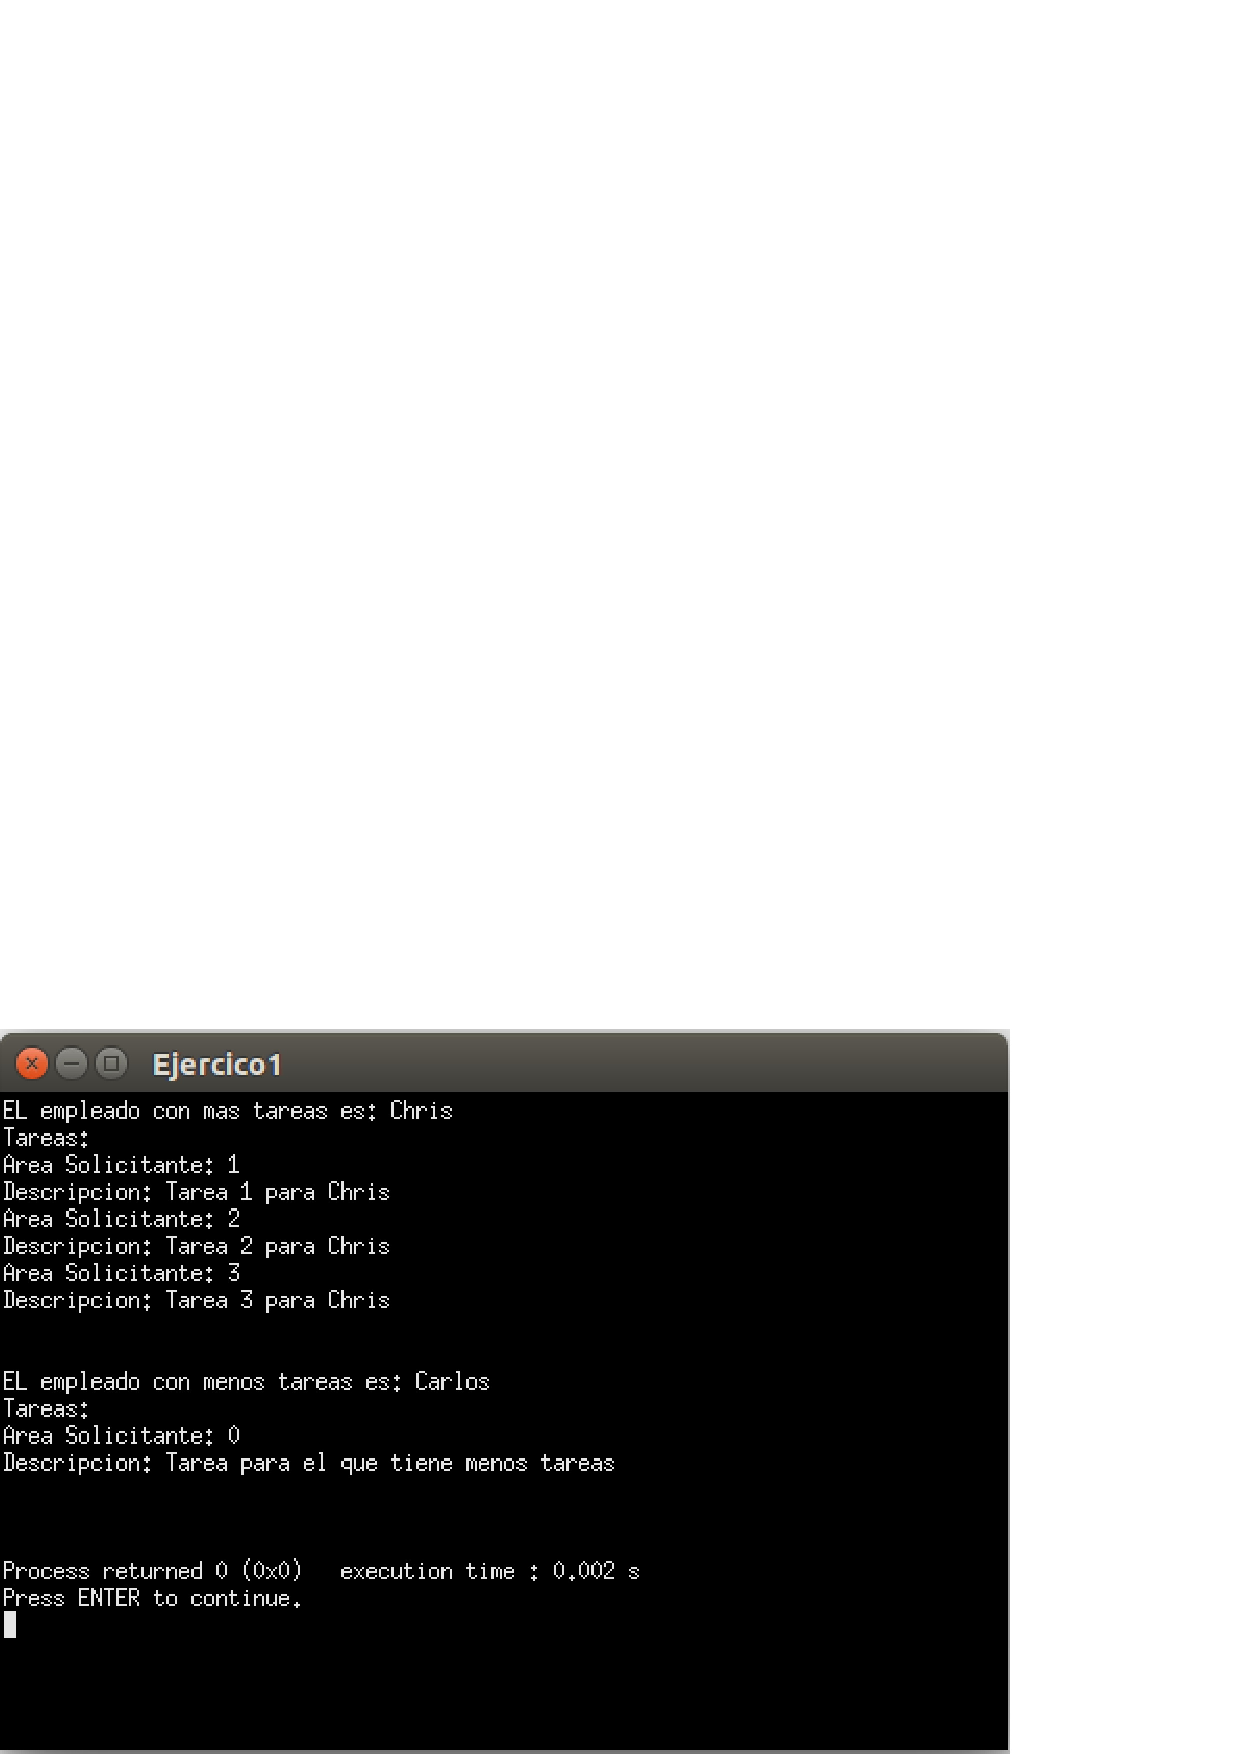
\includegraphics[scale = 0.5]{1.png}
   \caption{Resultados}
  \end{figure}
  
 \item \textbf{Implementar el método SCANLINE para el rellenado de polígonos}
 
 \begin{lstlisting}
 void fillFigureScanLine(Matrix matrix, int color){
    changeColor(color);
    bool flag = false;
    bool flag2 = false; // flag para pixeles seguidos
    for(int i = matrix.yMax - 1; i > matrix.yMin; i--){
        flag = false;
        for(int j = 0; j < matrix.size.width; j++){
            if(matrix.matrix[abs(i - matrix.size.height - 1)][j] == true){
                if(flag2 == false){
                    flag2 = true;
                    flag = !flag;
                }
            }
            else{
                if(flag == true){
                   setPixel(j,i);
                }
                if(flag2 == true) flag2 = false;
            }
            
        }
    }  
}
 \end{lstlisting}
 
 \begin{figure}[H]
  \centering
  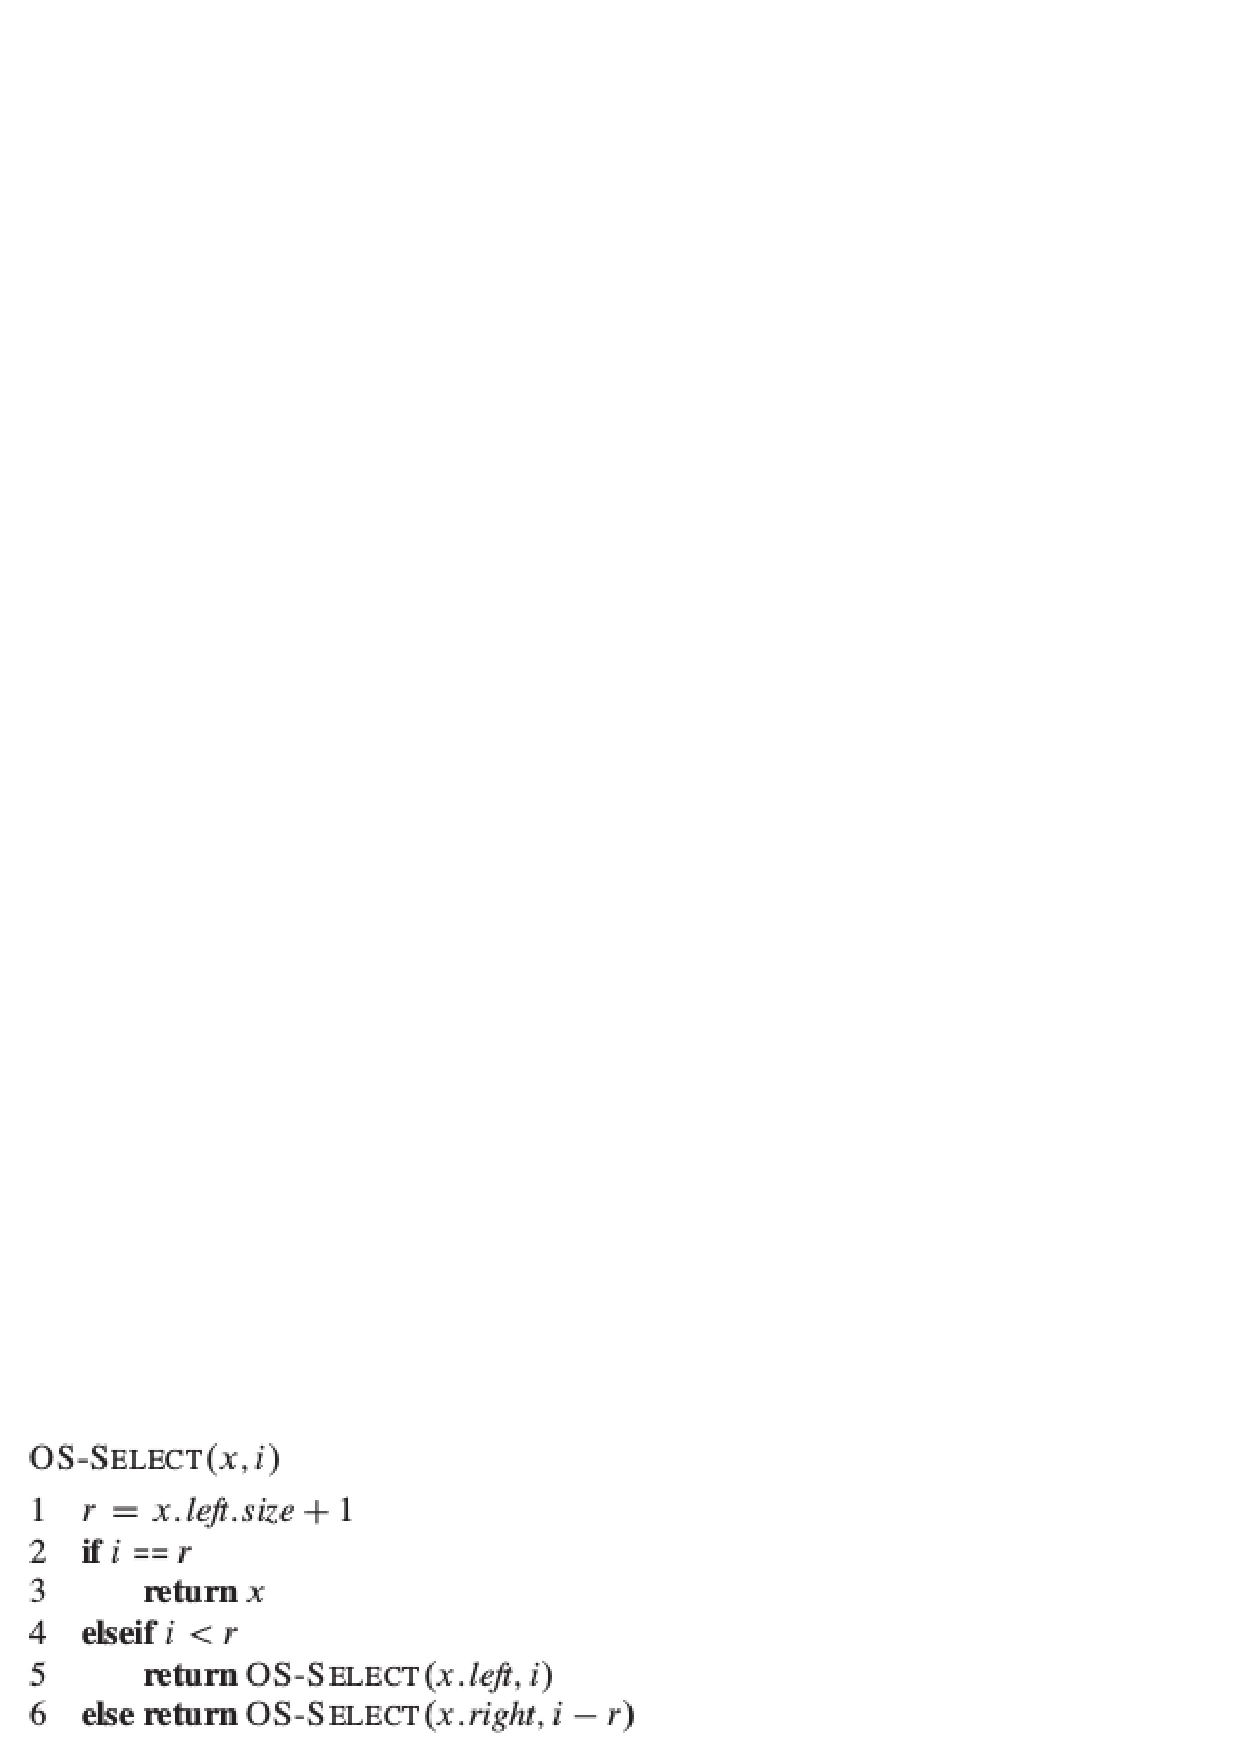
\includegraphics[scale = 0.5]{2.png}
  \caption{Resultados}
  
 \end{figure}


  

 
\end{enumerate}


\end{document}

